\begin{figure}[H]
    \centering
    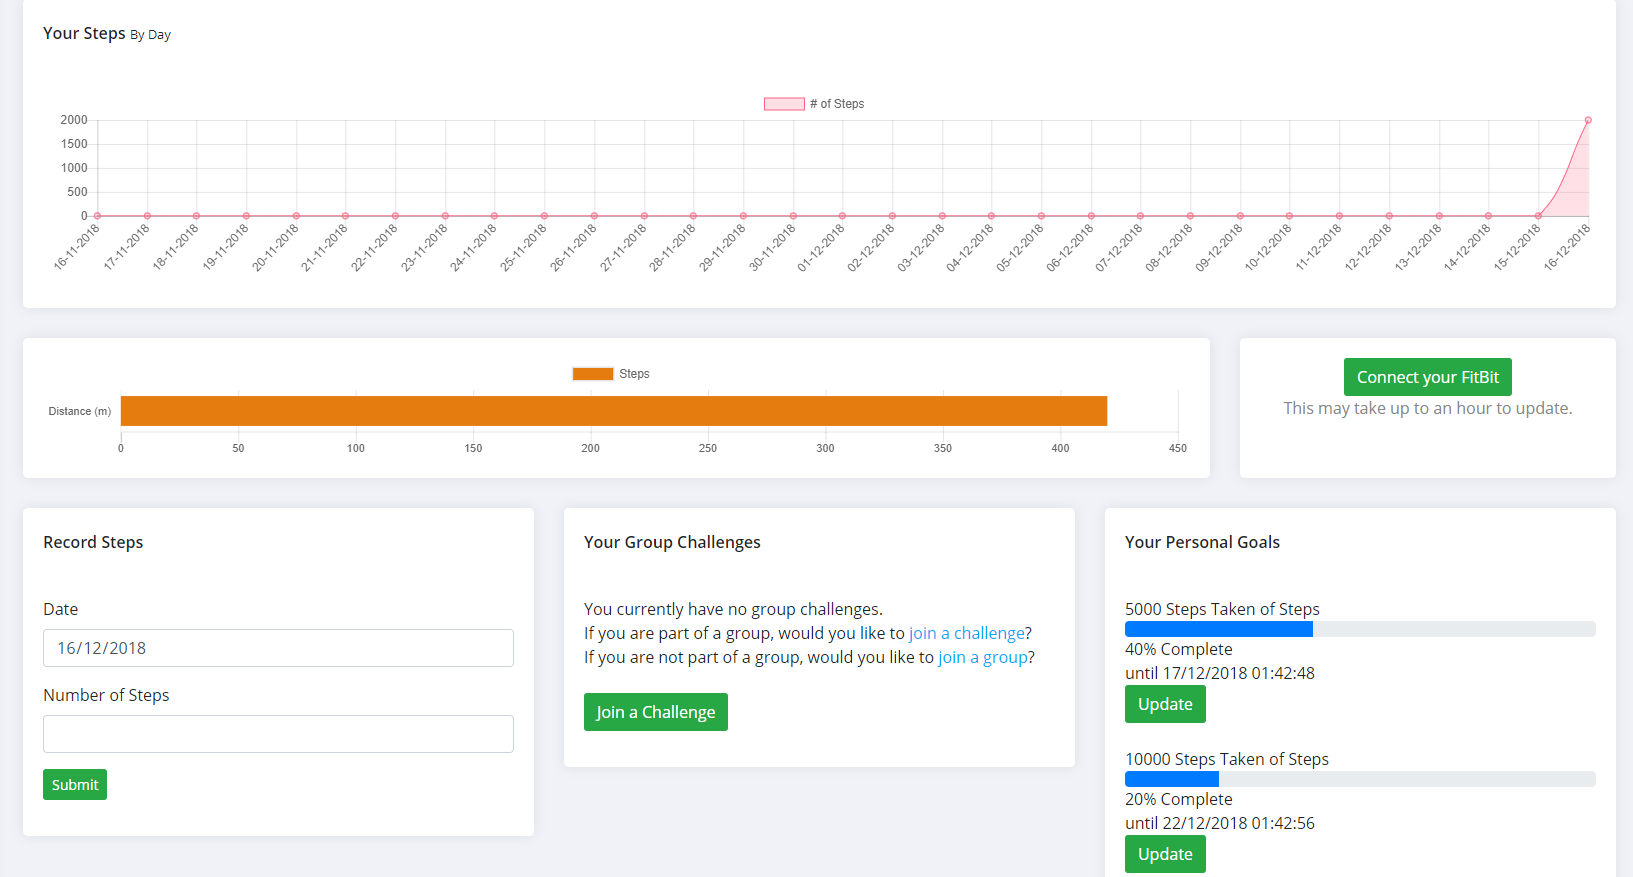
\includegraphics[width=\textwidth]{Images/service_dashboard.png}
    \caption{A screenshot showing a user accessing the main Dashboard, which is the view they are presented with when they first log into Aber Fitness}
\end{figure}

Please see acceptance test table in Appendix 2, Section 0.2.7.

Twelve acceptance tests were defined for the \textit{Health Dashboard} microservice, with one failing to pass. The failing test was one which required the user be able to specify a time frame when viewing their data. This functionality was not implemented in the final release.

In addition to the failing acceptance test, there are four outstanding issues with this microservice at time of release:

\begin{itemize}

	\item If no activity types are not defined within \textit{Health Data Repository}, the page will fail to load

	\item Rankings: user can only see rankings within their group, not ranking of their group within all groups
	
	\item Only number of steps is visualised from the activity metrics. Other metrics, such as Average Heart Rate and Calories Burnt, are not displayed

\end{itemize}